\section[Análise das Ferramentas]{Análise das Ferramentas}
Foram instaladas e testadas cada uma das ferramentas pesquisadas para que fosse decidido qual das três se adequasse melhor ao processo.

\subsection{Tiger Pro}
A instalação da ferramenta pode ser feita de maneira bem trivial, no entanto é necessária uma base de dados para que a ferramenta funcione. Essa necessidade pode ser suprida por meio do uso de um arquivo do tipo CSV ou utilizando uma base de dados MySQL ou Oracle, por exemplo.

A ferramenta tem quase 10 anos de lançamento, sem novas atualizações desde 2006. Possui interface um pouco confusa, mas aparentemente funcional. Dentre aos dados relacionadas com os requisitos, os mais importantes que a ferramenta permite o gerenciamento são:
\begin{itemize}
  \item Critérios de Aceitação;
  \item Análise Relacional ou Base Lógica;
  \item Rastreabilidade;
  \item Prioridade;
  \item Risco;
  \item Estimativa de Custos.
\end{itemize}

Dentre os atributos de requisitos que foram definidos para controlar e informar sobre os requisitos no projeto, apenas Prioridade foi encontrado na ferramenta.
A ferramenta permite o gerenciamento de outros atributos, porém estes outros não foram definidos previamente e nem observamos vantagens no seu uso para o projeto atual.
Por causa da limitação da ferramenta em relação aos atributos que ela controla e os atributos que escolhemos, e por ser uma ferramenta já descontinuada, a ferramenta não
se adequa ao processo definido.

\begin{figure}[!htb]
\centering
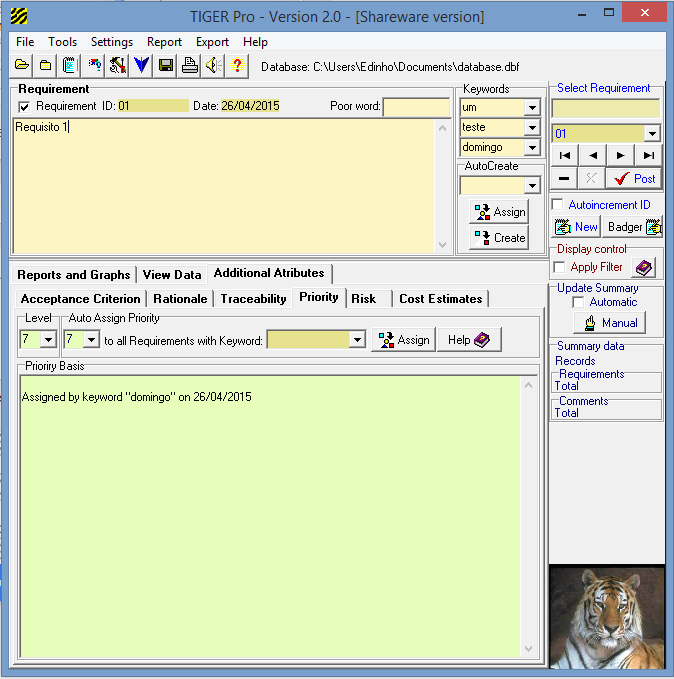
\includegraphics[scale=0.4]{figuras/tiger-pro.png}
\caption{Tela inicial da ferramenta Tiger-Pro}
\end{figure}

\subsection{TraceCloud}
Não há grandes problemas no que se refere a instalação da ferramenta, pois ela é \textit{online}. A ferramenta pode ser usada por um grupo de usuários e os dados da mesma podem ser alterados por todos os envolvidos no projeto. Uma das grandes desvantagens da ferramenta, se refere ao fato da mesma ser via \textit{Web}, ou seja, em locais em que não há acesso a internet, é impossível de se trabalhar.

A ferramenta vai de encontro com o que o grupo definiu como atributos de estudo, pois ela registra perfeitamente e de forma intuitiva as características dos requisitos que são gerenciadas pela mesma, algumas delas são:
\begin{itemize}
  \item Gerência de mudanças;
  \item Status de aprovação dos requisitos;
  \item Status de andamento das atividades envolvendo os requisitos;
  \item Prioridade no desenvolvimento dos requisitos;
  \item Requisitos relacionados.
\end{itemize}

O TraceCloud, fornece aos usuários uma divisão muito bem definida dos requisitos funcionais e dos de negócio por meio de pastas no canto esquerdo. Essas mesmas pastas possuem também uma área direcionada aos casos de testes que podem ser devidamente documentadas em um devido espaço.
Além disso, há a possibilidade de dividir algumas funções para membros do projeto e definir a data de entrega da mesma, o que é de grande valor para
qualquer projeto, criando uma espécie de agenda da equipe para as mais diversas iterações. Há a possibilidade do rastreamento do requisito desde sua criação,
até o mesmo ser desenvolvido por completo, além da possibilidade de vinculá-lo a um outro requisito.

\begin{figure}[!htb]
\centering
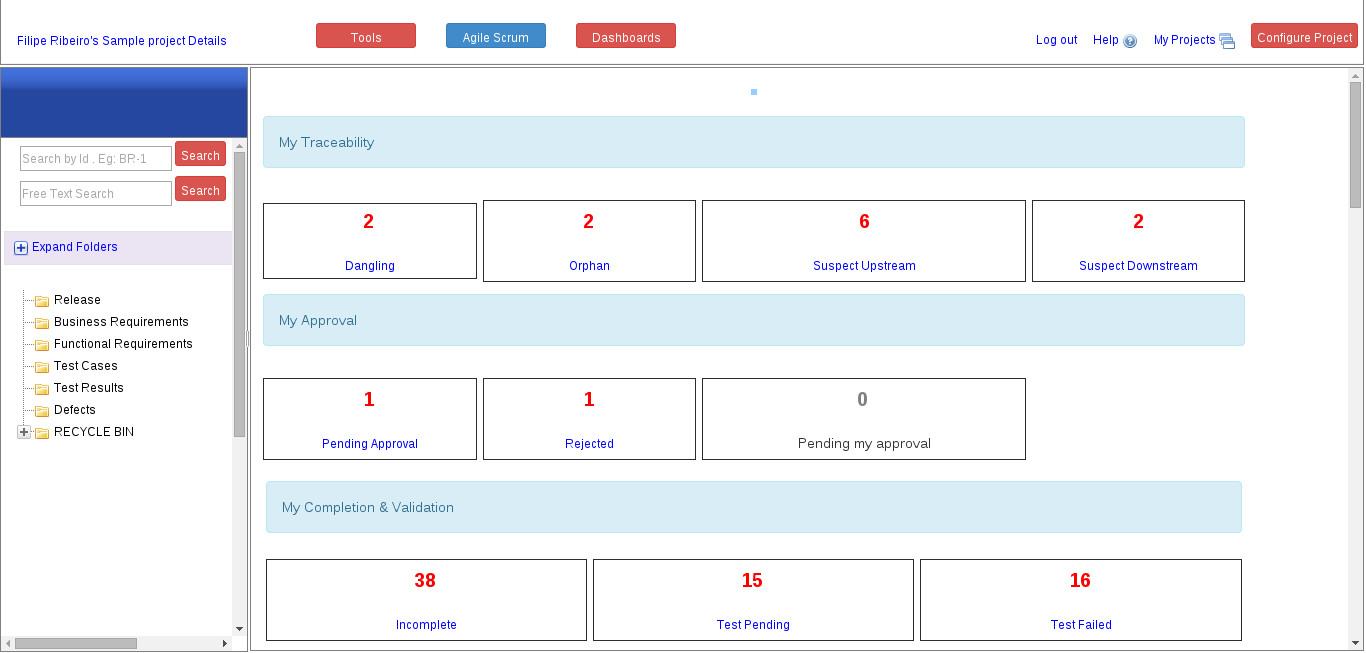
\includegraphics[scale=0.3]{figuras/trace.jpg}
\caption{Tela inicial da ferramenta TraceCloud}
\label{Rotulo}
\end{figure}

\subsection{Caliber}
A instalação da ferramenta é fácil, sendo necessário fazer um cadastro. A ferramenta é paga, mas possui a versão para testes por 30 dias.
Foi escolhida essa versão para avaliar a ferramenta.

A ferramenta gerencia muito bem os requisitos nos seguintes critérios:
\begin{itemize}
  \item Mudança dos requisitos;
  \item Prioridade dos requisitos;
  \item Rastreabilidade;
  \item Relacionamento dos requisitos;
  \item Análise dos requisitos.
\end{itemize}

Qualquer alteração que os requisitos sofrem é registrada pela ferramenta no histórico de mudanças a data e hora da mudança, o responsável e há
também a possibilidade de se fazer um comentário referente a tal mudança.

A organização dos itens da ferramenta usa um padrão já conhecido pelos usuários de outras ferramentas similares, barra a esquerda com os dados do projeto,
menu na barra superior. Isso torna a ferramenta fácil de usar, evitando que o usuário fique confuso.

\begin{figure}[!htb]
\centering
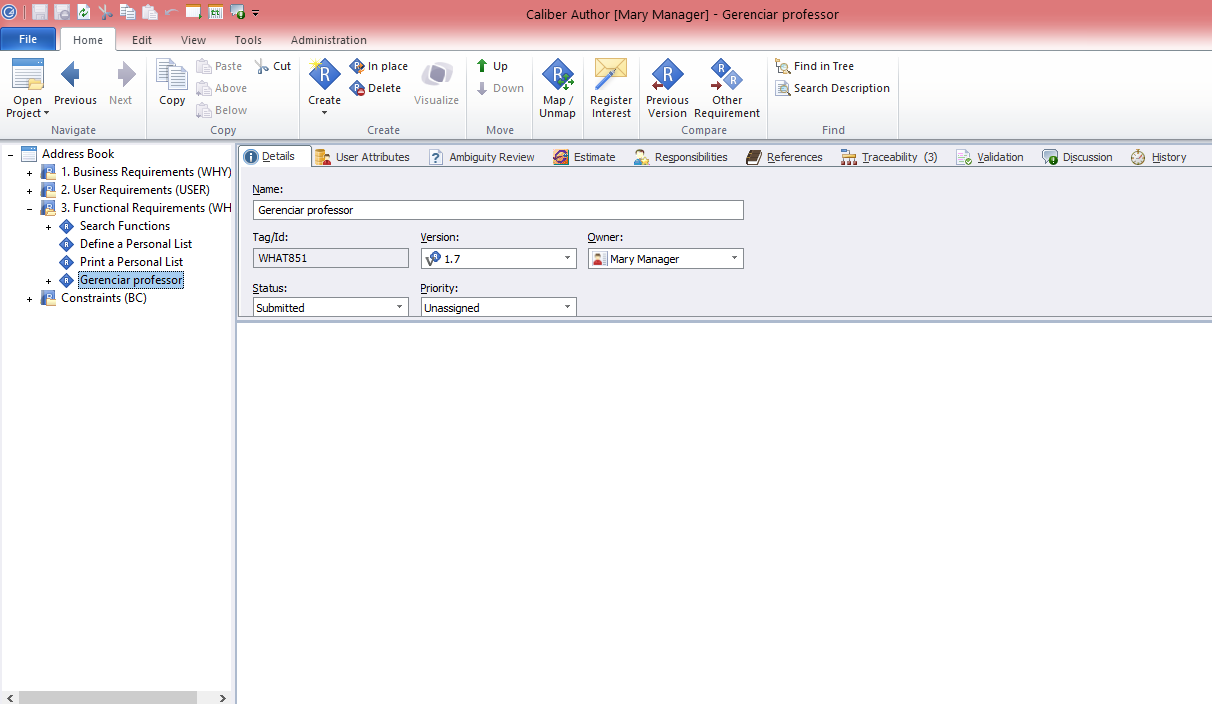
\includegraphics[scale=0.4]{figuras/caliber.png}
\caption{Tela inicial da ferramenta Caliber}
\end{figure}
